\subsubsection{Numerical experiments - Estimation of $\Phi$}

\textbf{Killing boundary conditions.} We consider the same simple case as in section \ref{sec:ExpTau2D} We consider $\partial D$ to be a killing boundary. The solution of \eqref{eq:GeneralModel} is in this case a Brownian motion. In this case, the partial differential equation \eqref{eq:PDEPhi} reduces to
\begin{equation}\label{eq:PDEPhi2DKilling}
\begin{cases}
	\frac{\partial}{\partial t} \Phi(x,t,T) + \frac{1}{2} \sigma^2 \Delta \Phi(x,t,T) = 0, & \text{in } D, \\
	\Phi(x,t,T) = 1, & \text{on } \partial D, \\
	\Phi(x,T,T) = 0, & \text{in } \partial D.
\end{cases}
\end{equation}
We solve this problem numerically with the Finite Elements Method as for \eqref{eq:PDETau2DKilling}. The solution at $t = 0$ is shown in Figure \ref{fig:PhiExact2DKill}. We verify the orders of convergence of DEM and CEM setting $X_0 = (0,0)^T , \sigma = 1, T = 0.5$. We consider $M = 100000$ trajectories and $N = 2^i,i=0,\dots,5$. We then compare the Montecarlo estimation with the value of $\Phi$ in $(0,0)$, obtained by interpolation on the Finite Elements solution. The orders of convergence for this numerical experiment are shown in Figure \ref{fig:KillTwoDPhi}. The theoretical orders of convergence are confirmed in this case as well, with an average order of $0.43$ for DEM and $1.19$ for CEM.

\begin{figure}[t]
    \centering
    \begin{subfigure}{0.49\linewidth}
        \centering
        \resizebox{1\linewidth}{!}{% This file was created by matlab2tikz.
%
%The latest updates can be retrieved from
%  http://www.mathworks.com/matlabcentral/fileexchange/22022-matlab2tikz-matlab2tikz
%where you can also make suggestions and rate matlab2tikz.
%
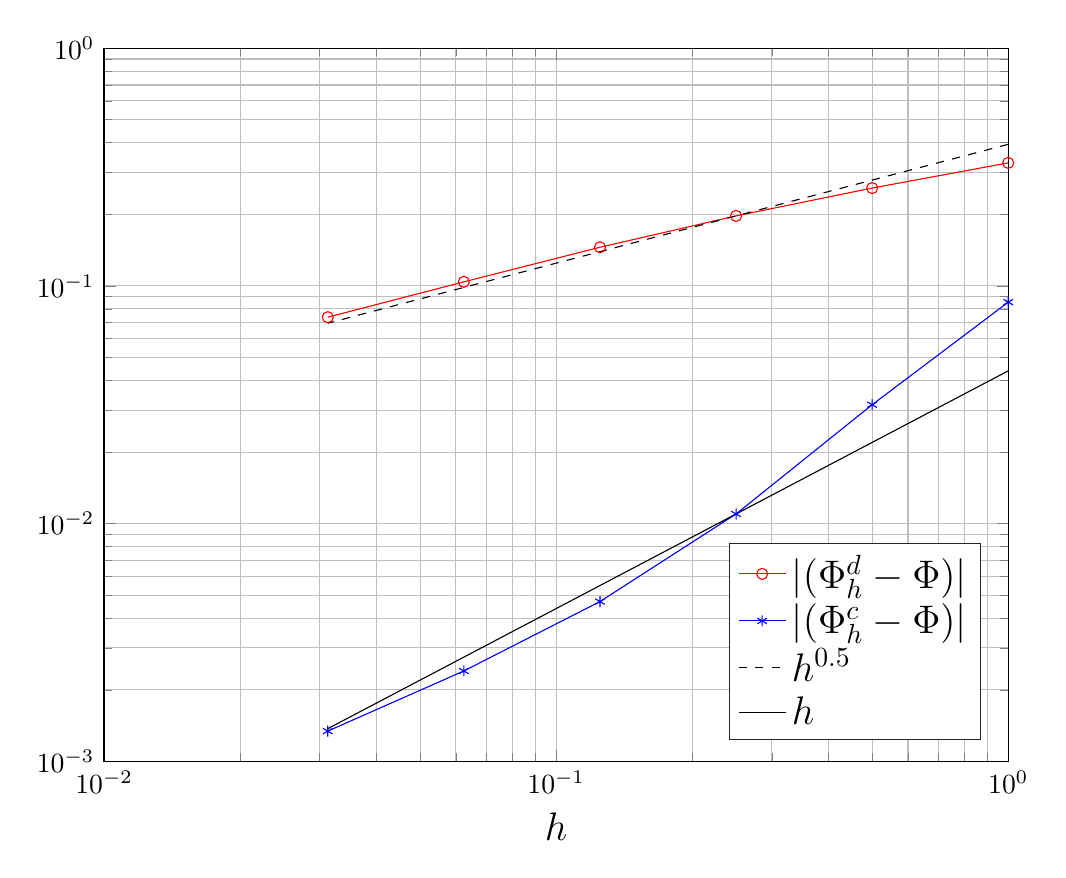
\begin{tikzpicture}

\begin{axis}[%
width=4.521in,
height=3.566in,
at={(0.758in,0.481in)},
scale only axis,
xmode=log,
xmin=0.01,
xmax=1,
xminorticks=true,
xlabel={$h$},
xlabel style={font=\Large},
xmajorgrids,
xminorgrids,
ymode=log,
ymin=0.001,
ymax=1,
yminorticks=true,
ymajorgrids,
yminorgrids,
axis background/.style={fill=white},
legend pos = south east,
legend style={legend cell align=left,align=left,draw=white!15!black,font=\Large}
]
\addplot [color=red,solid,mark=o,mark options={solid}]
  table[row sep=crcr]{%
1	0.329250554513686\\
0.5	0.257940554513686\\
0.25	0.197050554513686\\
0.125	0.145390554513686\\
0.0625	0.104000554513686\\
0.03125	0.073860554513686\\
};
\addlegendentry{$|\E(\Phi_h^d - \Phi)|$};

\addplot [color=blue,solid,mark=asterisk,mark options={solid}]
  table[row sep=crcr]{%
1	0.085450554513686\\
0.5	0.031640554513686\\
0.25	0.010980554513686\\
0.125	0.00470055451368601\\
0.0625	0.00240055451368593\\
0.03125	0.00134055451368598\\
};
\addlegendentry{$|\E(\Phi_h^c - \Phi)|$};

\addplot [color=black,dashed]
  table[row sep=crcr]{%
1	0.394101109027372\\
0.5	0.278671566666394\\
0.25	0.197050554513686\\
0.125	0.139335783333197\\
0.0625	0.098525277256843\\
0.03125	0.0696678916665984\\
};
\addlegendentry{$h^{0.5}$};

\addplot [color=black,solid]
  table[row sep=crcr]{%
1	0.0439222180547438\\
0.5	0.0219611090273719\\
0.25	0.010980554513686\\
0.125	0.00549027725684298\\
0.0625	0.00274513862842149\\
0.03125	0.00137256931421074\\
};
\addlegendentry{$h$};

\end{axis}
\end{tikzpicture}%
 }  
        \caption{Convergence of CEM and DEM.}
        \label{fig:KillTwoDPhi}
    \end{subfigure}
    \begin{subfigure}{0.49\linewidth}
        \centering
        \resizebox{1\linewidth}{!}{% This file was created by matlab2tikz.
%
%The latest updates can be retrieved from
%  http://www.mathworks.com/matlabcentral/fileexchange/22022-matlab2tikz-matlab2tikz
%where you can also make suggestions and rate matlab2tikz.
%
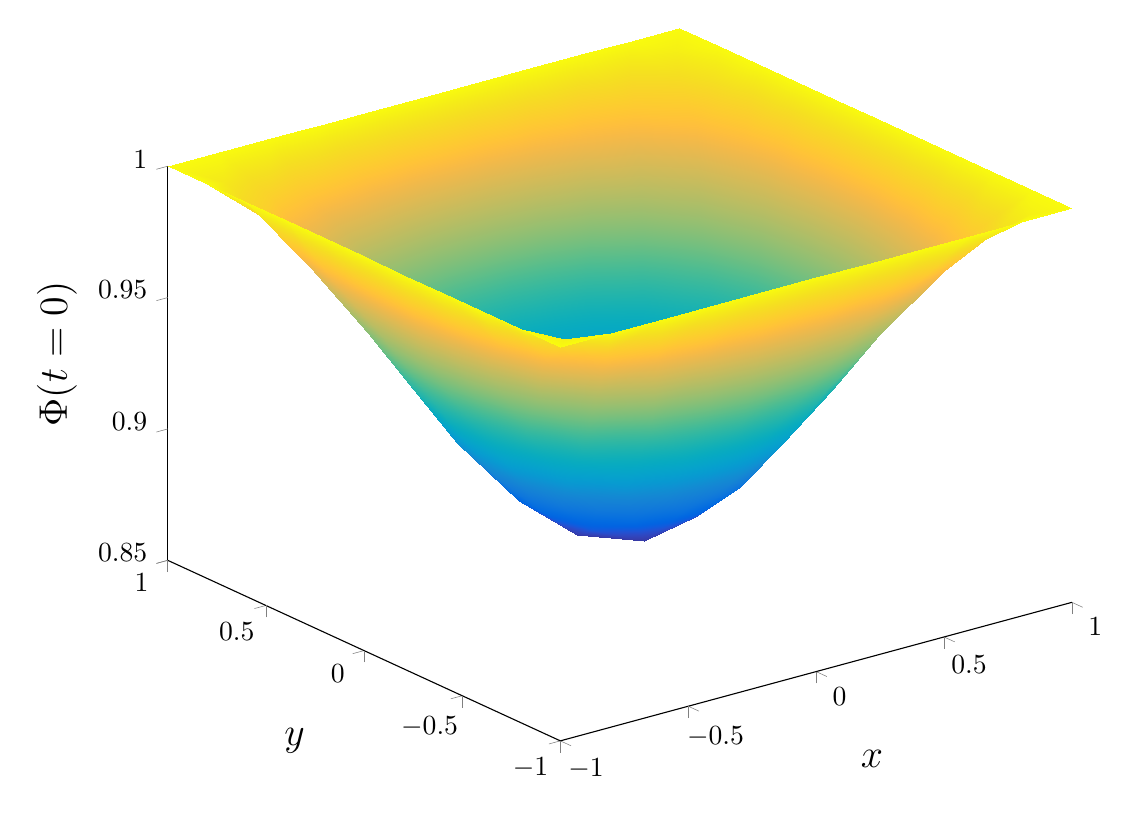
\begin{tikzpicture}

\begin{axis}[%
width=4.521in,
height=3.566in,
at={(0.758in,0.481in)},
scale only axis,
colormap={mymap}{[1pt] rgb(0pt)=(0.2081,0.1663,0.5292); rgb(1pt)=(0.211624,0.189781,0.577676); rgb(2pt)=(0.212252,0.213771,0.626971); rgb(3pt)=(0.2081,0.2386,0.677086); rgb(4pt)=(0.195905,0.264457,0.7279); rgb(5pt)=(0.170729,0.291938,0.779248); rgb(6pt)=(0.125271,0.324243,0.830271); rgb(7pt)=(0.0591333,0.359833,0.868333); rgb(8pt)=(0.0116952,0.38751,0.881957); rgb(9pt)=(0.00595714,0.408614,0.882843); rgb(10pt)=(0.0165143,0.4266,0.878633); rgb(11pt)=(0.0328524,0.443043,0.871957); rgb(12pt)=(0.0498143,0.458571,0.864057); rgb(13pt)=(0.0629333,0.47369,0.855438); rgb(14pt)=(0.0722667,0.488667,0.8467); rgb(15pt)=(0.0779429,0.503986,0.838371); rgb(16pt)=(0.0793476,0.520024,0.831181); rgb(17pt)=(0.0749429,0.537543,0.826271); rgb(18pt)=(0.0640571,0.556986,0.823957); rgb(19pt)=(0.0487714,0.577224,0.822829); rgb(20pt)=(0.0343429,0.596581,0.819852); rgb(21pt)=(0.0265,0.6137,0.8135); rgb(22pt)=(0.0238905,0.628662,0.803762); rgb(23pt)=(0.0230905,0.641786,0.791267); rgb(24pt)=(0.0227714,0.653486,0.776757); rgb(25pt)=(0.0266619,0.664195,0.760719); rgb(26pt)=(0.0383714,0.674271,0.743552); rgb(27pt)=(0.0589714,0.683757,0.725386); rgb(28pt)=(0.0843,0.692833,0.706167); rgb(29pt)=(0.113295,0.7015,0.685857); rgb(30pt)=(0.145271,0.709757,0.664629); rgb(31pt)=(0.180133,0.717657,0.642433); rgb(32pt)=(0.217829,0.725043,0.619262); rgb(33pt)=(0.258643,0.731714,0.595429); rgb(34pt)=(0.302171,0.737605,0.571186); rgb(35pt)=(0.348167,0.742433,0.547267); rgb(36pt)=(0.395257,0.7459,0.524443); rgb(37pt)=(0.44201,0.748081,0.503314); rgb(38pt)=(0.487124,0.749062,0.483976); rgb(39pt)=(0.530029,0.749114,0.466114); rgb(40pt)=(0.570857,0.748519,0.44939); rgb(41pt)=(0.609852,0.747314,0.433686); rgb(42pt)=(0.6473,0.7456,0.4188); rgb(43pt)=(0.683419,0.743476,0.404433); rgb(44pt)=(0.71841,0.741133,0.390476); rgb(45pt)=(0.752486,0.7384,0.376814); rgb(46pt)=(0.785843,0.735567,0.363271); rgb(47pt)=(0.818505,0.732733,0.34979); rgb(48pt)=(0.850657,0.7299,0.336029); rgb(49pt)=(0.882433,0.727433,0.3217); rgb(50pt)=(0.913933,0.725786,0.306276); rgb(51pt)=(0.944957,0.726114,0.288643); rgb(52pt)=(0.973895,0.731395,0.266648); rgb(53pt)=(0.993771,0.745457,0.240348); rgb(54pt)=(0.999043,0.765314,0.216414); rgb(55pt)=(0.995533,0.786057,0.196652); rgb(56pt)=(0.988,0.8066,0.179367); rgb(57pt)=(0.978857,0.827143,0.163314); rgb(58pt)=(0.9697,0.848138,0.147452); rgb(59pt)=(0.962586,0.870514,0.1309); rgb(60pt)=(0.958871,0.8949,0.113243); rgb(61pt)=(0.959824,0.921833,0.0948381); rgb(62pt)=(0.9661,0.951443,0.0755333); rgb(63pt)=(0.9763,0.9831,0.0538)},
xmin=-1,
xmax=1,
tick align=outside,
xlabel={$x$},
xlabel style = {font=\Large},
ymin=-1,
ymax=1,
ylabel={$y$},
ylabel style={font=\Large},
zmin=0.85,
zmax=1,
zlabel={$\Phi(t=0)$},
zlabel style={font=\Large},
view={-37.5}{30},
axis background/.style={fill=white},
axis x line*=bottom,
axis y line*=left,
axis z line*=left
]

\addplot3[area legend,solid,table/row sep=crcr,patch,shader=interp,forget plot,patch table={%
0	1	2\\
3	4	5\\
6	7	8\\
9	10	11\\
12	13	14\\
15	16	17\\
18	19	20\\
21	22	23\\
24	25	26\\
27	28	29\\
30	31	32\\
33	34	35\\
36	37	38\\
39	40	41\\
42	43	44\\
45	46	47\\
48	49	50\\
51	52	53\\
54	55	56\\
57	58	59\\
60	61	62\\
63	64	65\\
66	67	68\\
69	70	71\\
72	73	74\\
75	76	77\\
78	79	80\\
81	82	83\\
84	85	86\\
87	88	89\\
90	91	92\\
93	94	95\\
96	97	98\\
99	100	101\\
102	103	104\\
105	106	107\\
108	109	110\\
111	112	113\\
114	115	116\\
117	118	119\\
120	121	122\\
123	124	125\\
126	127	128\\
129	130	131\\
132	133	134\\
135	136	137\\
138	139	140\\
141	142	143\\
144	145	146\\
147	148	149\\
150	151	152\\
153	154	155\\
156	157	158\\
159	160	161\\
162	163	164\\
165	166	167\\
168	169	170\\
171	172	173\\
174	175	176\\
177	178	179\\
180	181	182\\
183	184	185\\
186	187	188\\
189	190	191\\
192	193	194\\
195	196	197\\
198	199	200\\
201	202	203\\
204	205	206\\
207	208	209\\
210	211	212\\
213	214	215\\
216	217	218\\
219	220	221\\
222	223	224\\
225	226	227\\
228	229	230\\
231	232	233\\
234	235	236\\
237	238	239\\
240	241	242\\
243	244	245\\
246	247	248\\
249	250	251\\
252	253	254\\
255	256	257\\
258	259	260\\
261	262	263\\
264	265	266\\
267	268	269\\
270	271	272\\
273	274	275\\
276	277	278\\
279	280	281\\
282	283	284\\
285	286	287\\
288	289	290\\
291	292	293\\
294	295	296\\
297	298	299\\
300	301	302\\
303	304	305\\
306	307	308\\
309	310	311\\
312	313	314\\
315	316	317\\
318	319	320\\
321	322	323\\
324	325	326\\
327	328	329\\
330	331	332\\
333	334	335\\
336	337	338\\
339	340	341\\
342	343	344\\
345	346	347\\
348	349	350\\
351	352	353\\
354	355	356\\
357	358	359\\
360	361	362\\
363	364	365\\
366	367	368\\
369	370	371\\
372	373	374\\
375	376	377\\
378	379	380\\
381	382	383\\
384	385	386\\
387	388	389\\
390	391	392\\
393	394	395\\
396	397	398\\
399	400	401\\
402	403	404\\
405	406	407\\
408	409	410\\
411	412	413\\
414	415	416\\
417	418	419\\
420	421	422\\
423	424	425\\
426	427	428\\
429	430	431\\
432	433	434\\
435	436	437\\
438	439	440\\
441	442	443\\
444	445	446\\
447	448	449\\
450	451	452\\
453	454	455\\
456	457	458\\
459	460	461\\
462	463	464\\
465	466	467\\
468	469	470\\
471	472	473\\
474	475	476\\
477	478	479\\
480	481	482\\
483	484	485\\
486	487	488\\
489	490	491\\
492	493	494\\
495	496	497\\
498	499	500\\
501	502	503\\
504	505	506\\
507	508	509\\
510	511	512\\
513	514	515\\
516	517	518\\
519	520	521\\
522	523	524\\
525	526	527\\
528	529	530\\
531	532	533\\
534	535	536\\
537	538	539\\
540	541	542\\
543	544	545\\
546	547	548\\
549	550	551\\
552	553	554\\
555	556	557\\
558	559	560\\
561	562	563\\
564	565	566\\
567	568	569\\
570	571	572\\
573	574	575\\
576	577	578\\
579	580	581\\
582	583	584\\
585	586	587\\
588	589	590\\
591	592	593\\
594	595	596\\
597	598	599\\
600	601	602\\
603	604	605\\
606	607	608\\
609	610	611\\
612	613	614\\
615	616	617\\
618	619	620\\
621	622	623\\
624	625	626\\
627	628	629\\
630	631	632\\
633	634	635\\
636	637	638\\
639	640	641\\
642	643	644\\
645	646	647\\
648	649	650\\
651	652	653\\
654	655	656\\
657	658	659\\
660	661	662\\
663	664	665\\
666	667	668\\
669	670	671\\
672	673	674\\
675	676	677\\
678	679	680\\
681	682	683\\
684	685	686\\
687	688	689\\
690	691	692\\
693	694	695\\
696	697	698\\
699	700	701\\
702	703	704\\
705	706	707\\
708	709	710\\
711	712	713\\
714	715	716\\
717	718	719\\
720	721	722\\
723	724	725\\
726	727	728\\
729	730	731\\
732	733	734\\
735	736	737\\
738	739	740\\
741	742	743\\
744	745	746\\
747	748	749\\
750	751	752\\
753	754	755\\
756	757	758\\
759	760	761\\
762	763	764\\
765	766	767\\
768	769	770\\
771	772	773\\
774	775	776\\
777	778	779\\
780	781	782\\
783	784	785\\
786	787	788\\
789	790	791\\
792	793	794\\
795	796	797\\
798	799	800\\
801	802	803\\
804	805	806\\
807	808	809\\
810	811	812\\
813	814	815\\
816	817	818\\
819	820	821\\
822	823	824\\
825	826	827\\
828	829	830\\
831	832	833\\
834	835	836\\
837	838	839\\
840	841	842\\
843	844	845\\
846	847	848\\
849	850	851\\
852	853	854\\
855	856	857\\
858	859	860\\
861	862	863\\
864	865	866\\
867	868	869\\
870	871	872\\
873	874	875\\
876	877	878\\
879	880	881\\
882	883	884\\
885	886	887\\
888	889	890\\
891	892	893\\
894	895	896\\
897	898	899\\
900	901	902\\
903	904	905\\
906	907	908\\
909	910	911\\
912	913	914\\
915	916	917\\
918	919	920\\
921	922	923\\
924	925	926\\
927	928	929\\
930	931	932\\
933	934	935\\
}]
table[row sep=crcr, point meta=\thisrow{c}] {%
x	y	z	c\\
-0.8	1	1	1\\
-1	1	1	1\\
-0.870979864217162	0.874090623781756	0.994900837726379	0.994900837726379\\
-0.6	1	1	1\\
-0.8	1	1	1\\
-0.715759069893515	0.851783447512538	0.98676550492405	0.98676550492405\\
-0.4	1	1	1\\
-0.6	1	1	1\\
-0.553557227232278	0.85599352174284	0.98067301275533	0.98067301275533\\
-0.2	1	1	1\\
-0.4	1	1	1\\
-0.256371139537587	0.844436132195903	0.970613925501264	0.970613925501264\\
0	1	1	1\\
-0.2	1	1	1\\
-0.123171927132804	0.882407229449651	0.976271284529154	0.976271284529154\\
0.2	1	1	1\\
0	1	1	1\\
0.138576080047019	0.836444863570092	0.96718109036119	0.96718109036119\\
0.4	1	1	1\\
0.2	1	1	1\\
0.314746867281053	0.841650113118016	0.971244672546017	0.971244672546017\\
0.6	1	1	1\\
0.4	1	1	1\\
0.500557557249754	0.834821560479383	0.975897428674888	0.975897428674888\\
1	0.8	1	1\\
1	1	1	1\\
0.913245437763783	0.903908655259532	0.997293344589815	0.997293344589815\\
0.8	1	1	1\\
0.6	1	1	1\\
0.6908636124721	0.827426566529025	0.983406646219684	0.983406646219684\\
1	1	1	1\\
0.8	1	1	1\\
0.913245437763783	0.903908655259532	0.997293344589815	0.997293344589815\\
0.913245437763783	0.903908655259532	0.997293344589815	0.997293344589815\\
0.8	1	1	1\\
0.853111865010539	0.81689479082676	0.991331631283587	0.991331631283587\\
1	0.6	1	1\\
1	0.8	1	1\\
0.913257156072776	0.71766207885242	0.992249980519293	0.992249980519293\\
1	0.4	1	1\\
1	0.6	1	1\\
0.858172452446661	0.489687445107711	0.978931416261557	0.978931416261557\\
1	0.2	1	1\\
1	0.4	1	1\\
0.801876020058965	0.306586241275605	0.963819950493757	0.963819950493757\\
1	-0.2	1	1\\
1	0	1	1\\
0.842830738889788	-0.109162193087545	0.968151883748015	0.968151883748015\\
1	-0.4	1	1\\
1	-0.2	1	1\\
0.839553137409186	-0.294644298019888	0.970332773422549	0.970332773422549\\
1	-0.6	1	1\\
1	-0.4	1	1\\
0.825961266928206	-0.490102064147121	0.974309290789402	0.974309290789402\\
0.8	-1	1	1\\
1	-1	1	1\\
0.903543131650638	-0.913183857559471	0.997280162089009	0.997280162089009\\
1	-0.8	1	1\\
1	-0.6	1	1\\
0.822757598423982	-0.688930059869196	0.982870705844679	0.982870705844679\\
1	-1	1	1\\
1	-0.8	1	1\\
0.903543131650638	-0.913183857559471	0.997280162089009	0.997280162089009\\
0.903543131650638	-0.913183857559471	0.997280162089009	0.997280162089009\\
1	-0.8	1	1\\
0.815246907920555	-0.852962033044177	0.991224519889577	0.991224519889577\\
0.6	-1	1	1\\
0.8	-1	1	1\\
0.716262971529556	-0.913440138799354	0.992201811500356	0.992201811500356\\
0.4	-1	1	1\\
0.6	-1	1	1\\
0.486610676987292	-0.860815662729556	0.979180011966515	0.979180011966515\\
0.2	-1	1	1\\
0.4	-1	1	1\\
0.30415666992098	-0.806486553345674	0.964572648989551	0.964572648989551\\
-0.2	-1	1	1\\
0	-1	1	1\\
-0.108836774839956	-0.842631178463089	0.968104206702289	0.968104206702289\\
-0.4	-1	1	1\\
-0.2	-1	1	1\\
-0.295155054484333	-0.839202734226978	0.970290719712475	0.970290719712475\\
-0.6	-1	1	1\\
-0.4	-1	1	1\\
-0.491181950150036	-0.827450133500077	0.974605590135046	0.974605590135046\\
-1	-0.8	1	1\\
-1	-1	1	1\\
-0.913179600822541	-0.903978796898105	0.997285844316782	0.997285844316782\\
-0.8	-1	1	1\\
-0.6	-1	1	1\\
-0.689383148912005	-0.825669061227738	0.983178068811281	0.983178068811281\\
-1	-1	1	1\\
-0.8	-1	1	1\\
-0.913179600822541	-0.903978796898105	0.997285844316782	0.997285844316782\\
-0.913179600822541	-0.903978796898105	0.997285844316782	0.997285844316782\\
-0.8	-1	1	1\\
-0.852930471573381	-0.817084814175369	0.99130925528688	0.99130925528688\\
-1	-0.6	1	1\\
-1	-0.8	1	1\\
-0.913349182557632	-0.71824277938499	0.992270278388791	0.992270278388791\\
-1	-0.4	1	1\\
-1	-0.6	1	1\\
-0.858612569930114	-0.502582179815703	0.97936622817875	0.97936622817875\\
-1	-0.2	1	1\\
-1	-0.4	1	1\\
-0.875147249859378	-0.2495178793164	0.976260703864056	0.976260703864056\\
0.822757598423982	-0.688930059869196	0.982870705844679	0.982870705844679\\
1	-0.6	1	1\\
0.825961266928206	-0.490102064147121	0.974309290789402	0.974309290789402\\
-1	0.2	1	1\\
-1	0	1	1\\
-0.878430687062504	0.0687937548368703	0.97513912998771	0.97513912998771\\
-1	0.4	1	1\\
-1	0.2	1	1\\
-0.858638192546528	0.336283758462884	0.974938148517588	0.974938148517588\\
0.314746867281053	0.841650113118016	0.971244672546017	0.971244672546017\\
0.2	1	1	1\\
0.138576080047019	0.836444863570092	0.96718109036119	0.96718109036119\\
-1	0.6	1	1\\
-1	0.4	1	1\\
-0.81542002432126	0.514265339146589	0.973484087503461	0.973484087503461\\
-1	0	1	1\\
-1	-0.2	1	1\\
-0.849550627410001	-0.0857161204413969	0.969276748763463	0.969276748763463\\
-0.81542002432126	0.514265339146589	0.973484087503461	0.973484087503461\\
-1	0.4	1	1\\
-0.858638192546528	0.336283758462884	0.974938148517588	0.974938148517588\\
0	-1	1	1\\
0.2	-1	1	1\\
0.0842448278397462	-0.826656651009239	0.964646736627235	0.964646736627235\\
-0.295155054484333	-0.839202734226978	0.970290719712475	0.970290719712475\\
-0.2	-1	1	1\\
-0.108836774839956	-0.842631178463089	0.968104206702289	0.968104206702289\\
1	0	1	1\\
1	0.2	1	1\\
0.825000730866433	0.0840636812185947	0.964317376856716	0.964317376856716\\
0.839553137409186	-0.294644298019888	0.970332773422549	0.970332773422549\\
1	-0.2	1	1\\
0.842830738889788	-0.109162193087545	0.968151883748015	0.968151883748015\\
-0.421476522111469	0.76529746608585	0.962144255721489	0.962144255721489\\
-0.4	1	1	1\\
-0.553557227232278	0.85599352174284	0.98067301275533	0.98067301275533\\
-1	1	1	1\\
-1	0.8	1	1\\
-0.870979864217162	0.874090623781756	0.994900837726379	0.994900837726379\\
-1	0.8	1	1\\
-1	0.6	1	1\\
-0.838909094432717	0.717165597536304	0.985693767813085	0.985693767813085\\
-0.870979864217162	0.874090623781756	0.994900837726379	0.994900837726379\\
-1	0.8	1	1\\
-0.838909094432717	0.717165597536304	0.985693767813085	0.985693767813085\\
-0.689383148912005	-0.825669061227738	0.983178068811281	0.983178068811281\\
-0.6	-1	1	1\\
-0.491181950150036	-0.827450133500077	0.974605590135046	0.974605590135046\\
0.162899107774523	0.0782930267751429	0.872742439565376	0.872742439565376\\
-0.0145232187187818	0.0259493451768655	0.867789035029159	0.867789035029159\\
0.0995954131227801	-0.0711056079718885	0.870504568793608	0.870504568793608\\
0.6908636124721	0.827426566529025	0.983406646219684	0.983406646219684\\
0.6	1	1	1\\
0.500557557249754	0.834821560479383	0.975897428674888	0.975897428674888\\
-0.0437189086592884	-0.1794562797288	0.87256194036436	0.87256194036436\\
-0.0145232187187818	0.0259493451768655	0.867789035029159	0.867789035029159\\
-0.183666461200581	-0.0196981175980336	0.873147501411437	0.873147501411437\\
-0.183666461200581	-0.0196981175980336	0.873147501411437	0.873147501411437\\
-0.0145232187187818	0.0259493451768655	0.867789035029159	0.867789035029159\\
-0.143244730260345	0.15312684048721	0.8747397674553	0.8747397674553\\
-0.573742666641828	0.478792000601255	0.94013688725324	0.94013688725324\\
-0.435775856529045	0.402580883145608	0.917493027129057	0.917493027129057\\
-0.436448993108287	0.574739898722634	0.936632614165645	0.936632614165645\\
-0.777645420963466	0.191713474052978	0.9567401595428	0.9567401595428\\
-1	0.2	1	1\\
-0.878430687062504	0.0687937548368703	0.97513912998771	0.97513912998771\\
-0.308985524220196	-0.434191396690207	0.90902950197148	0.90902950197148\\
-0.44256229481138	-0.30475784338953	0.909723124538403	0.909723124538403\\
-0.504626867096141	-0.476494146294975	0.93173214285744	0.93173214285744\\
0.30415666992098	-0.806486553345674	0.964572648989551	0.964572648989551\\
0.4	-1	1	1\\
0.486610676987292	-0.860815662729556	0.979180011966515	0.979180011966515\\
0.0893690793198263	-0.463478876426208	0.90220023494353	0.90220023494353\\
0.261928641455601	-0.488055957894452	0.912657925264648	0.912657925264648\\
0.2060410026947	-0.342035240885369	0.892345370672627	0.892345370672627\\
0.801876020058965	0.306586241275605	0.963819950493757	0.963819950493757\\
1	0.4	1	1\\
0.858172452446661	0.489687445107711	0.978931416261557	0.978931416261557\\
0.500557557249754	0.834821560479383	0.975897428674888	0.975897428674888\\
0.4	1	1	1\\
0.314746867281053	0.841650113118016	0.971244672546017	0.971244672546017\\
-0.0174658545926647	0.801898927302032	0.959585165793654	0.959585165793654\\
0	1	1	1\\
-0.123171927132804	0.882407229449651	0.976271284529154	0.976271284529154\\
0.629591208237007	0.150059132096618	0.929130478486791	0.929130478486791\\
0.464005364535939	0.260203010616371	0.909336169977326	0.909336169977326\\
0.457941066948159	0.074681360252563	0.901147721016767	0.901147721016767\\
-0.536183382478912	-0.125067364855863	0.913131201655364	0.913131201655364\\
-0.44256229481138	-0.30475784338953	0.909723124538403	0.909723124538403\\
-0.376489904228021	-0.187383275146088	0.895309106052268	0.895309106052268\\
0.825961266928206	-0.490102064147121	0.974309290789402	0.974309290789402\\
1	-0.4	1	1\\
0.839553137409186	-0.294644298019888	0.970332773422549	0.970332773422549\\
-0.491181950150036	-0.827450133500077	0.974605590135046	0.974605590135046\\
-0.4	-1	1	1\\
-0.295155054484333	-0.839202734226978	0.970290719712475	0.970290719712475\\
0.151932036409303	-0.636460365815934	0.930371299389602	0.930371299389602\\
0.261928641455601	-0.488055957894452	0.912657925264648	0.912657925264648\\
0.0893690793198263	-0.463478876426208	0.90220023494353	0.90220023494353\\
-0.31111533158028	-0.281732042536466	0.894897915733725	0.894897915733725\\
-0.241660277500026	-0.172513969577467	0.881749240369071	0.881749240369071\\
-0.376489904228021	-0.187383275146088	0.895309106052268	0.895309106052268\\
-0.796122724389227	-0.361886425045465	0.964838218238696	0.964838218238696\\
-0.695084883753552	-0.495926997595022	0.956478867662404	0.956478867662404\\
-0.617615903555302	-0.32670910304294	0.934719729982011	0.934719729982011\\
0.321736948673632	-0.218404805181936	0.890932340087552	0.890932340087552\\
0.149400916774043	-0.200302697508326	0.877738679478757	0.877738679478757\\
0.2060410026947	-0.342035240885369	0.892345370672627	0.892345370672627\\
0.459725917575231	0.478817132146761	0.927135234802201	0.927135234802201\\
0.464005364535939	0.260203010616371	0.909336169977326	0.909336169977326\\
0.609248416595618	0.336700564235885	0.934184498196784	0.934184498196784\\
-0.591992818593216	-0.654470500305776	0.958999843467768	0.958999843467768\\
-0.368952164395011	-0.646051178924541	0.941319463263012	0.941319463263012\\
-0.504626867096141	-0.476494146294975	0.93173214285744	0.93173214285744\\
0.646526572158138	-0.5892372548303	0.957861085974691	0.957861085974691\\
0.647783933105589	-0.365727428795828	0.941322680027829	0.941322680027829\\
0.453484147433517	-0.490455219207141	0.927783458305522	0.927783458305522\\
-0.8	1	1	1\\
-0.870979864217162	0.874090623781756	0.994900837726379	0.994900837726379\\
-0.715759069893515	0.851783447512538	0.98676550492405	0.98676550492405\\
-0.436448993108287	0.574739898722634	0.936632614165645	0.936632614165645\\
-0.435775856529045	0.402580883145608	0.917493027129057	0.917493027129057\\
-0.305196827885855	0.481941510996423	0.914960284883457	0.914960284883457\\
0.651531723544283	-0.800304145152872	0.978288699073484	0.978288699073484\\
0.6	-1	1	1\\
0.716262971529556	-0.913440138799354	0.992201811500356	0.992201811500356\\
0.651531723544283	-0.800304145152872	0.978288699073484	0.978288699073484\\
0.822757598423982	-0.688930059869196	0.982870705844679	0.982870705844679\\
0.646526572158138	-0.5892372548303	0.957861085974691	0.957861085974691\\
0.457941066948159	0.074681360252563	0.901147721016767	0.901147721016767\\
0.464005364535939	0.260203010616371	0.909336169977326	0.909336169977326\\
0.313359205867812	0.176240487473655	0.887896532202356	0.887896532202356\\
0.799426193403826	0.656174087711846	0.978483640300531	0.978483640300531\\
1	0.6	1	1\\
0.913257156072776	0.71766207885242	0.992249980519293	0.992249980519293\\
-0.800381152695487	-0.658205081403852	0.978683809212969	0.978683809212969\\
-1	-0.6	1	1\\
-0.913349182557632	-0.71824277938499	0.992270278388791	0.992270278388791\\
-0.800381152695487	-0.658205081403852	0.978683809212969	0.978683809212969\\
-0.689383148912005	-0.825669061227738	0.983178068811281	0.983178068811281\\
-0.591992818593216	-0.654470500305776	0.958999843467768	0.958999843467768\\
-0.131538906378604	0.468005506270669	0.903630473858266	0.903630473858266\\
0.0468419620052357	0.523978954343319	0.910307614863627	0.910307614863627\\
-0.0677763280124889	0.648507972991784	0.930995342052713	0.930995342052713\\
0.172508063347201	0.422930104621211	0.899727098372923	0.899727098372923\\
0.0468419620052357	0.523978954343319	0.910307614863627	0.910307614863627\\
0.0285171270359044	0.362157622648837	0.888681212576899	0.888681212576899\\
0.453484147433517	-0.490455219207141	0.927783458305522	0.927783458305522\\
0.261928641455601	-0.488055957894452	0.912657925264648	0.912657925264648\\
0.32991065048365	-0.623943472007708	0.935962241356271	0.935962241356271\\
0.0893690793198263	-0.463478876426208	0.90220023494353	0.90220023494353\\
-0.0468923144628943	-0.37201189317892	0.890086243397066	0.890086243397066\\
-0.0519572972000214	-0.516668038614571	0.90947302329719	0.90947302329719\\
0.801876020058965	0.306586241275605	0.963819950493757	0.963819950493757\\
0.687082418720278	0.487393175878324	0.954672383311247	0.954672383311247\\
0.609248416595618	0.336700564235885	0.934184498196784	0.934184498196784\\
0.457941066948159	0.074681360252563	0.901147721016767	0.901147721016767\\
0.386220146013541	-0.0691483215457924	0.892145935388779	0.892145935388779\\
0.521855887175084	-0.0613271652026621	0.910406355736384	0.910406355736384\\
0.0893728715906334	0.678554065055819	0.936706510961468	0.936706510961468\\
0.0468419620052357	0.523978954343319	0.910307614863627	0.910307614863627\\
0.193142943255321	0.563632036809665	0.920225864035588	0.920225864035588\\
-0.467792458521678	0.219937427890346	0.907318261019031	0.907318261019031\\
-0.435775856529045	0.402580883145608	0.917493027129057	0.917493027129057\\
-0.560240270361451	0.344844062180542	0.928151038726253	0.928151038726253\\
0.0172621493060368	0.196448852647962	0.874027891656812	0.874027891656812\\
0.167453556422288	0.263155683226473	0.883029460766085	0.883029460766085\\
0.0285171270359044	0.362157622648837	0.888681212576899	0.888681212576899\\
-0.777645420963466	0.191713474052978	0.9567401595428	0.9567401595428\\
-0.617913717697813	0.079971000861777	0.925668535700939	0.925668535700939\\
-0.624616411644707	0.242665578371416	0.932057644027081	0.932057644027081\\
-0.536183382478912	-0.125067364855863	0.913131201655364	0.913131201655364\\
-0.617913717697813	0.079971000861777	0.925668535700939	0.925668535700939\\
-0.699519166874299	-0.0584145433376073	0.940247517792943	0.940247517792943\\
-0.421476522111469	0.76529746608585	0.962144255721489	0.962144255721489\\
-0.629666025324687	0.659481894250005	0.962502195017753	0.962502195017753\\
-0.436448993108287	0.574739898722634	0.936632614165645	0.936632614165645\\
-0.467792458521678	0.219937427890346	0.907318261019031	0.907318261019031\\
-0.617913717697813	0.079971000861777	0.925668535700939	0.925668535700939\\
-0.456541297467842	0.0462574378515442	0.900794951092116	0.900794951092116\\
-0.796122724389227	-0.361886425045465	0.964838218238696	0.964838218238696\\
-1	-0.4	1	1\\
-0.858612569930114	-0.502582179815703	0.97936622817875	0.97936622817875\\
0.30415666992098	-0.806486553345674	0.964572648989551	0.964572648989551\\
0.478214140797659	-0.695585476223675	0.955154623786944	0.955154623786944\\
0.32991065048365	-0.623943472007708	0.935962241356271	0.935962241356271\\
-0.350427977113875	-0.0568798710953585	0.88776979894399	0.88776979894399\\
-0.241660277500026	-0.172513969577467	0.881749240369071	0.881749240369071\\
-0.183666461200581	-0.0196981175980336	0.873147501411437	0.873147501411437\\
0.521855887175084	-0.0613271652026621	0.910406355736384	0.910406355736384\\
0.386220146013541	-0.0691483215457924	0.892145935388779	0.892145935388779\\
0.456651668322266	-0.168447833276863	0.904183192578576	0.904183192578576\\
-0.256371139537587	0.844436132195903	0.970613925501264	0.970613925501264\\
-0.251840934393812	0.65073582839654	0.936254830816768	0.936254830816768\\
-0.14310781983293	0.765817634248709	0.953814782517273	0.953814782517273\\
1	0.8	1	1\\
0.913245437763783	0.903908655259532	0.997293344589815	0.997293344589815\\
0.853111865010539	0.81689479082676	0.991331631283587	0.991331631283587\\
-0.131538906378604	0.468005506270669	0.903630473858266	0.903630473858266\\
-0.0999792356165469	0.29750658388758	0.883678609501141	0.883678609501141\\
0.0285171270359044	0.362157622648837	0.888681212576899	0.888681212576899\\
0.799426193403826	0.656174087711846	0.978483640300531	0.978483640300531\\
0.687082418720278	0.487393175878324	0.954672383311247	0.954672383311247\\
0.858172452446661	0.489687445107711	0.978931416261557	0.978931416261557\\
0.239679041234336	-0.0747988778282174	0.877981689297287	0.877981689297287\\
0.386220146013541	-0.0691483215457924	0.892145935388779	0.892145935388779\\
0.312829618686655	0.0361464359017708	0.883951433224601	0.883951433224601\\
0.651531723544283	-0.800304145152872	0.978288699073484	0.978288699073484\\
0.478214140797659	-0.695585476223675	0.955154623786944	0.955154623786944\\
0.486610676987292	-0.860815662729556	0.979180011966515	0.979180011966515\\
-0.0437189086592884	-0.1794562797288	0.87256194036436	0.87256194036436\\
-0.0468923144628943	-0.37201189317892	0.890086243397066	0.890086243397066\\
0.0706839927525276	-0.312287735493971	0.884388922846536	0.884388922846536\\
-0.617615903555302	-0.32670910304294	0.934719729982011	0.934719729982011\\
-0.695084883753552	-0.495926997595022	0.956478867662404	0.956478867662404\\
-0.504626867096141	-0.476494146294975	0.93173214285744	0.93173214285744\\
-0.308985524220196	-0.434191396690207	0.90902950197148	0.90902950197148\\
-0.368952164395011	-0.646051178924541	0.941319463263012	0.941319463263012\\
-0.188699779816531	-0.572089273359516	0.921238008263871	0.921238008263871\\
0.467892646677106	-0.300972929247376	0.912829432030675	0.912829432030675\\
0.647783933105589	-0.365727428795828	0.941322680027829	0.941322680027829\\
0.581538749766835	-0.190353470678335	0.922862308308852	0.922862308308852\\
0.321736948673632	-0.218404805181936	0.890932340087552	0.890932340087552\\
0.386220146013541	-0.0691483215457924	0.892145935388779	0.892145935388779\\
0.239679041234336	-0.0747988778282174	0.877981689297287	0.877981689297287\\
0.6908636124721	0.827426566529025	0.983406646219684	0.983406646219684\\
0.500557557249754	0.834821560479383	0.975897428674888	0.975897428674888\\
0.590963022235164	0.660549521945042	0.959569544566287	0.959569544566287\\
0.590963022235164	0.660549521945042	0.959569544566287	0.959569544566287\\
0.500557557249754	0.834821560479383	0.975897428674888	0.975897428674888\\
0.404778435204039	0.681910640519122	0.948759865781375	0.948759865781375\\
-0.838909094432717	0.717165597536304	0.985693767813085	0.985693767813085\\
-1	0.6	1	1\\
-0.81542002432126	0.514265339146589	0.973484087503461	0.973484087503461\\
-0.573742666641828	0.478792000601255	0.94013688725324	0.94013688725324\\
-0.629666025324687	0.659481894250005	0.962502195017753	0.962502195017753\\
-0.67998691843914	0.507882653342416	0.955894223829624	0.955894223829624\\
-1	-0.8	1	1\\
-0.913179600822541	-0.903978796898105	0.997285844316782	0.997285844316782\\
-0.852930471573381	-0.817084814175369	0.99130925528688	0.99130925528688\\
-0.491181950150036	-0.827450133500077	0.974605590135046	0.974605590135046\\
-0.368952164395011	-0.646051178924541	0.941319463263012	0.941319463263012\\
-0.591992818593216	-0.654470500305776	0.958999843467768	0.958999843467768\\
0.590963022235164	0.660549521945042	0.959569544566287	0.959569544566287\\
0.687082418720278	0.487393175878324	0.954672383311247	0.954672383311247\\
0.799426193403826	0.656174087711846	0.978483640300531	0.978483640300531\\
0.6908636124721	0.827426566529025	0.983406646219684	0.983406646219684\\
0.590963022235164	0.660549521945042	0.959569544566287	0.959569544566287\\
0.799426193403826	0.656174087711846	0.978483640300531	0.978483640300531\\
0.8	-1	1	1\\
0.903543131650638	-0.913183857559471	0.997280162089009	0.997280162089009\\
0.815246907920555	-0.852962033044177	0.991224519889577	0.991224519889577\\
0.825961266928206	-0.490102064147121	0.974309290789402	0.974309290789402\\
0.647783933105589	-0.365727428795828	0.941322680027829	0.941322680027829\\
0.646526572158138	-0.5892372548303	0.957861085974691	0.957861085974691\\
-0.188699779816531	-0.572089273359516	0.921238008263871	0.921238008263871\\
-0.368952164395011	-0.646051178924541	0.941319463263012	0.941319463263012\\
-0.201012514379659	-0.715085349646872	0.945699896459097	0.945699896459097\\
-0.536183382478912	-0.125067364855863	0.913131201655364	0.913131201655364\\
-0.729105054552535	-0.200822554621074	0.948021711447488	0.948021711447488\\
-0.617615903555302	-0.32670910304294	0.934719729982011	0.934719729982011\\
0.581538749766835	-0.190353470678335	0.922862308308852	0.922862308308852\\
0.647783933105589	-0.365727428795828	0.941322680027829	0.941322680027829\\
0.717419694116031	-0.201076983778939	0.946122979608639	0.946122979608639\\
0.151932036409303	-0.636460365815934	0.930371299389602	0.930371299389602\\
0.30415666992098	-0.806486553345674	0.964572648989551	0.964572648989551\\
0.32991065048365	-0.623943472007708	0.935962241356271	0.935962241356271\\
-0.0519572972000214	-0.516668038614571	0.90947302329719	0.90947302329719\\
-0.0468923144628943	-0.37201189317892	0.890086243397066	0.890086243397066\\
-0.156991111184629	-0.442497792882714	0.901868922732904	0.901868922732904\\
-0.31111533158028	-0.281732042536466	0.894897915733725	0.894897915733725\\
-0.308985524220196	-0.434191396690207	0.90902950197148	0.90902950197148\\
-0.185241010817594	-0.314270126024311	0.888585716364086	0.888585716364086\\
-0.467792458521678	0.219937427890346	0.907318261019031	0.907318261019031\\
-0.311591314295825	0.109324344546677	0.884909589552814	0.884909589552814\\
-0.270562051272334	0.305759011517556	0.8926630123459	0.8926630123459\\
0.162899107774523	0.0782930267751429	0.872742439565376	0.872742439565376\\
0.167453556422288	0.263155683226473	0.883029460766085	0.883029460766085\\
0.0172621493060368	0.196448852647962	0.874027891656812	0.874027891656812\\
0.629591208237007	0.150059132096618	0.929130478486791	0.929130478486791\\
0.801876020058965	0.306586241275605	0.963819950493757	0.963819950493757\\
0.609248416595618	0.336700564235885	0.934184498196784	0.934184498196784\\
0.314746867281053	0.841650113118016	0.971244672546017	0.971244672546017\\
0.243215438556557	0.696935801995676	0.943802218859768	0.943802218859768\\
0.404778435204039	0.681910640519122	0.948759865781375	0.948759865781375\\
-0.421476522111469	0.76529746608585	0.962144255721489	0.962144255721489\\
-0.251840934393812	0.65073582839654	0.936254830816768	0.936254830816768\\
-0.256371139537587	0.844436132195903	0.970613925501264	0.970613925501264\\
0.404778435204039	0.681910640519122	0.948759865781375	0.948759865781375\\
0.243215438556557	0.696935801995676	0.943802218859768	0.943802218859768\\
0.318221535321866	0.579996560046282	0.929012104045419	0.929012104045419\\
0.581538749766835	-0.190353470678335	0.922862308308852	0.922862308308852\\
0.671060117555799	-0.0425238644998574	0.934737906860778	0.934737906860778\\
0.521855887175084	-0.0613271652026621	0.910406355736384	0.910406355736384\\
0.842830738889788	-0.109162193087545	0.968151883748015	0.968151883748015\\
1	0	1	1\\
0.825000730866433	0.0840636812185947	0.964317376856716	0.964317376856716\\
-0.188699779816531	-0.572089273359516	0.921238008263871	0.921238008263871\\
-0.0400681817402094	-0.67007462624905	0.934519728244642	0.934519728244642\\
-0.0519572972000214	-0.516668038614571	0.90947302329719	0.90947302329719\\
-0.108836774839956	-0.842631178463089	0.968104206702289	0.968104206702289\\
0	-1	1	1\\
0.0842448278397462	-0.826656651009239	0.964646736627235	0.964646736627235\\
-0.838909094432717	0.717165597536304	0.985693767813085	0.985693767813085\\
-0.629666025324687	0.659481894250005	0.962502195017753	0.962502195017753\\
-0.715759069893515	0.851783447512538	0.98676550492405	0.98676550492405\\
-0.131538906378604	0.468005506270669	0.903630473858266	0.903630473858266\\
-0.251840934393812	0.65073582839654	0.936254830816768	0.936254830816768\\
-0.305196827885855	0.481941510996423	0.914960284883457	0.914960284883457\\
-0.573742666641828	0.478792000601255	0.94013688725324	0.94013688725324\\
-0.698784277302622	0.374550558446254	0.949904646247805	0.949904646247805\\
-0.560240270361451	0.344844062180542	0.928151038726253	0.928151038726253\\
-0.849550627410001	-0.0857161204413969	0.969276748763463	0.969276748763463\\
-1	-0.2	1	1\\
-0.875147249859378	-0.2495178793164	0.976260703864056	0.976260703864056\\
0.629591208237007	0.150059132096618	0.929130478486791	0.929130478486791\\
0.671060117555799	-0.0425238644998574	0.934737906860778	0.934737906860778\\
0.825000730866433	0.0840636812185947	0.964317376856716	0.964317376856716\\
0.647783933105589	-0.365727428795828	0.941322680027829	0.941322680027829\\
0.825961266928206	-0.490102064147121	0.974309290789402	0.974309290789402\\
0.839553137409186	-0.294644298019888	0.970332773422549	0.970332773422549\\
0.151932036409303	-0.636460365815934	0.930371299389602	0.930371299389602\\
-0.0400681817402094	-0.67007462624905	0.934519728244642	0.934519728244642\\
0.0842448278397462	-0.826656651009239	0.964646736627235	0.964646736627235\\
-0.368952164395011	-0.646051178924541	0.941319463263012	0.941319463263012\\
-0.491181950150036	-0.827450133500077	0.974605590135046	0.974605590135046\\
-0.295155054484333	-0.839202734226978	0.970290719712475	0.970290719712475\\
-0.849550627410001	-0.0857161204413969	0.969276748763463	0.969276748763463\\
-0.729105054552535	-0.200822554621074	0.948021711447488	0.948021711447488\\
-0.699519166874299	-0.0584145433376073	0.940247517792943	0.940247517792943\\
-0.270562051272334	0.305759011517556	0.8926630123459	0.8926630123459\\
-0.311591314295825	0.109324344546677	0.884909589552814	0.884909589552814\\
-0.143244730260345	0.15312684048721	0.8747397674553	0.8747397674553\\
-0.44256229481138	-0.30475784338953	0.909723124538403	0.909723124538403\\
-0.308985524220196	-0.434191396690207	0.90902950197148	0.90902950197148\\
-0.31111533158028	-0.281732042536466	0.894897915733725	0.894897915733725\\
-0.251840934393812	0.65073582839654	0.936254830816768	0.936254830816768\\
-0.421476522111469	0.76529746608585	0.962144255721489	0.962144255721489\\
-0.436448993108287	0.574739898722634	0.936632614165645	0.936632614165645\\
-0.0437189086592884	-0.1794562797288	0.87256194036436	0.87256194036436\\
0.149400916774043	-0.200302697508326	0.877738679478757	0.877738679478757\\
0.0995954131227801	-0.0711056079718885	0.870504568793608	0.870504568793608\\
0.459725917575231	0.478817132146761	0.927135234802201	0.927135234802201\\
0.29046632350991	0.478227595927983	0.913486484415046	0.913486484415046\\
0.311159739978053	0.346682633914339	0.900187637296798	0.900187637296798\\
-0.695084883753552	-0.495926997595022	0.956478867662404	0.956478867662404\\
-0.800381152695487	-0.658205081403852	0.978683809212969	0.978683809212969\\
-0.591992818593216	-0.654470500305776	0.958999843467768	0.958999843467768\\
-0.689383148912005	-0.825669061227738	0.983178068811281	0.983178068811281\\
-0.491181950150036	-0.827450133500077	0.974605590135046	0.974605590135046\\
-0.591992818593216	-0.654470500305776	0.958999843467768	0.958999843467768\\
0.478214140797659	-0.695585476223675	0.955154623786944	0.955154623786944\\
0.651531723544283	-0.800304145152872	0.978288699073484	0.978288699073484\\
0.646526572158138	-0.5892372548303	0.957861085974691	0.957861085974691\\
0.822757598423982	-0.688930059869196	0.982870705844679	0.982870705844679\\
0.825961266928206	-0.490102064147121	0.974309290789402	0.974309290789402\\
0.646526572158138	-0.5892372548303	0.957861085974691	0.957861085974691\\
-0.777645420963466	0.191713474052978	0.9567401595428	0.9567401595428\\
-0.698784277302622	0.374550558446254	0.949904646247805	0.949904646247805\\
-0.858638192546528	0.336283758462884	0.974938148517588	0.974938148517588\\
-0.629666025324687	0.659481894250005	0.962502195017753	0.962502195017753\\
-0.838909094432717	0.717165597536304	0.985693767813085	0.985693767813085\\
-0.81542002432126	0.514265339146589	0.973484087503461	0.973484087503461\\
-0.870979864217162	0.874090623781756	0.994900837726379	0.994900837726379\\
-0.838909094432717	0.717165597536304	0.985693767813085	0.985693767813085\\
-0.715759069893515	0.851783447512538	0.98676550492405	0.98676550492405\\
-0.715759069893515	0.851783447512538	0.98676550492405	0.98676550492405\\
-0.629666025324687	0.659481894250005	0.962502195017753	0.962502195017753\\
-0.553557227232278	0.85599352174284	0.98067301275533	0.98067301275533\\
-0.44256229481138	-0.30475784338953	0.909723124538403	0.909723124538403\\
-0.536183382478912	-0.125067364855863	0.913131201655364	0.913131201655364\\
-0.617615903555302	-0.32670910304294	0.934719729982011	0.934719729982011\\
-0.800381152695487	-0.658205081403852	0.978683809212969	0.978683809212969\\
-0.695084883753552	-0.495926997595022	0.956478867662404	0.956478867662404\\
-0.858612569930114	-0.502582179815703	0.97936622817875	0.97936622817875\\
-0.698784277302622	0.374550558446254	0.949904646247805	0.949904646247805\\
-0.777645420963466	0.191713474052978	0.9567401595428	0.9567401595428\\
-0.624616411644707	0.242665578371416	0.932057644027081	0.932057644027081\\
-0.81542002432126	0.514265339146589	0.973484087503461	0.973484087503461\\
-0.698784277302622	0.374550558446254	0.949904646247805	0.949904646247805\\
-0.67998691843914	0.507882653342416	0.955894223829624	0.955894223829624\\
-0.617913717697813	0.079971000861777	0.925668535700939	0.925668535700939\\
-0.777645420963466	0.191713474052978	0.9567401595428	0.9567401595428\\
-0.764656987373661	0.0391649423298058	0.952429628969232	0.952429628969232\\
-0.796122724389227	-0.361886425045465	0.964838218238696	0.964838218238696\\
-0.729105054552535	-0.200822554621074	0.948021711447488	0.948021711447488\\
-0.875147249859378	-0.2495178793164	0.976260703864056	0.976260703864056\\
0.321736948673632	-0.218404805181936	0.890932340087552	0.890932340087552\\
0.467892646677106	-0.300972929247376	0.912829432030675	0.912829432030675\\
0.456651668322266	-0.168447833276863	0.904183192578576	0.904183192578576\\
0.842830738889788	-0.109162193087545	0.968151883748015	0.968151883748015\\
0.671060117555799	-0.0425238644998574	0.934737906860778	0.934737906860778\\
0.717419694116031	-0.201076983778939	0.946122979608639	0.946122979608639\\
-0.185241010817594	-0.314270126024311	0.888585716364086	0.888585716364086\\
-0.308985524220196	-0.434191396690207	0.90902950197148	0.90902950197148\\
-0.156991111184629	-0.442497792882714	0.901868922732904	0.901868922732904\\
-0.108836774839956	-0.842631178463089	0.968104206702289	0.968104206702289\\
-0.0400681817402094	-0.67007462624905	0.934519728244642	0.934519728244642\\
-0.201012514379659	-0.715085349646872	0.945699896459097	0.945699896459097\\
0.2	-1	1	1\\
0.30415666992098	-0.806486553345674	0.964572648989551	0.964572648989551\\
0.0842448278397462	-0.826656651009239	0.964646736627235	0.964646736627235\\
-0.368952164395011	-0.646051178924541	0.941319463263012	0.941319463263012\\
-0.295155054484333	-0.839202734226978	0.970290719712475	0.970290719712475\\
-0.201012514379659	-0.715085349646872	0.945699896459097	0.945699896459097\\
1	0.2	1	1\\
0.801876020058965	0.306586241275605	0.963819950493757	0.963819950493757\\
0.825000730866433	0.0840636812185947	0.964317376856716	0.964317376856716\\
0.647783933105589	-0.365727428795828	0.941322680027829	0.941322680027829\\
0.839553137409186	-0.294644298019888	0.970332773422549	0.970332773422549\\
0.717419694116031	-0.201076983778939	0.946122979608639	0.946122979608639\\
0.459725917575231	0.478817132146761	0.927135234802201	0.927135234802201\\
0.590963022235164	0.660549521945042	0.959569544566287	0.959569544566287\\
0.404778435204039	0.681910640519122	0.948759865781375	0.948759865781375\\
0.172508063347201	0.422930104621211	0.899727098372923	0.899727098372923\\
0.29046632350991	0.478227595927983	0.913486484415046	0.913486484415046\\
0.193142943255321	0.563632036809665	0.920225864035588	0.920225864035588\\
-0.368952164395011	-0.646051178924541	0.941319463263012	0.941319463263012\\
-0.308985524220196	-0.434191396690207	0.90902950197148	0.90902950197148\\
-0.504626867096141	-0.476494146294975	0.93173214285744	0.93173214285744\\
-0.729105054552535	-0.200822554621074	0.948021711447488	0.948021711447488\\
-0.796122724389227	-0.361886425045465	0.964838218238696	0.964838218238696\\
-0.617615903555302	-0.32670910304294	0.934719729982011	0.934719729982011\\
0.687082418720278	0.487393175878324	0.954672383311247	0.954672383311247\\
0.801876020058965	0.306586241275605	0.963819950493757	0.963819950493757\\
0.858172452446661	0.489687445107711	0.978931416261557	0.978931416261557\\
1	0.6	1	1\\
0.799426193403826	0.656174087711846	0.978483640300531	0.978483640300531\\
0.858172452446661	0.489687445107711	0.978931416261557	0.978931416261557\\
0.478214140797659	-0.695585476223675	0.955154623786944	0.955154623786944\\
0.30415666992098	-0.806486553345674	0.964572648989551	0.964572648989551\\
0.486610676987292	-0.860815662729556	0.979180011966515	0.979180011966515\\
0.6	-1	1	1\\
0.651531723544283	-0.800304145152872	0.978288699073484	0.978288699073484\\
0.486610676987292	-0.860815662729556	0.979180011966515	0.979180011966515\\
0.453484147433517	-0.490455219207141	0.927783458305522	0.927783458305522\\
0.467892646677106	-0.300972929247376	0.912829432030675	0.912829432030675\\
0.342470518429332	-0.368426311537438	0.905232183759213	0.905232183759213\\
0.0995954131227801	-0.0711056079718885	0.870504568793608	0.870504568793608\\
0.149400916774043	-0.200302697508326	0.877738679478757	0.877738679478757\\
0.239679041234336	-0.0747988778282174	0.877981689297287	0.877981689297287\\
-0.8	-1	1	1\\
-0.689383148912005	-0.825669061227738	0.983178068811281	0.983178068811281\\
-0.852930471573381	-0.817084814175369	0.99130925528688	0.99130925528688\\
-0.689383148912005	-0.825669061227738	0.983178068811281	0.983178068811281\\
-0.800381152695487	-0.658205081403852	0.978683809212969	0.978683809212969\\
-0.852930471573381	-0.817084814175369	0.99130925528688	0.99130925528688\\
0.8	1	1	1\\
0.6908636124721	0.827426566529025	0.983406646219684	0.983406646219684\\
0.853111865010539	0.81689479082676	0.991331631283587	0.991331631283587\\
0.6908636124721	0.827426566529025	0.983406646219684	0.983406646219684\\
0.799426193403826	0.656174087711846	0.978483640300531	0.978483640300531\\
0.853111865010539	0.81689479082676	0.991331631283587	0.991331631283587\\
1	-0.8	1	1\\
0.822757598423982	-0.688930059869196	0.982870705844679	0.982870705844679\\
0.815246907920555	-0.852962033044177	0.991224519889577	0.991224519889577\\
0.822757598423982	-0.688930059869196	0.982870705844679	0.982870705844679\\
0.651531723544283	-0.800304145152872	0.978288699073484	0.978288699073484\\
0.815246907920555	-0.852962033044177	0.991224519889577	0.991224519889577\\
0.0172621493060368	0.196448852647962	0.874027891656812	0.874027891656812\\
-0.0999792356165469	0.29750658388758	0.883678609501141	0.883678609501141\\
-0.143244730260345	0.15312684048721	0.8747397674553	0.8747397674553\\
0.0893728715906334	0.678554065055819	0.936706510961468	0.936706510961468\\
-0.0174658545926647	0.801898927302032	0.959585165793654	0.959585165793654\\
-0.0677763280124889	0.648507972991784	0.930995342052713	0.930995342052713\\
0.30415666992098	-0.806486553345674	0.964572648989551	0.964572648989551\\
0.151932036409303	-0.636460365815934	0.930371299389602	0.930371299389602\\
0.0842448278397462	-0.826656651009239	0.964646736627235	0.964646736627235\\
-0.0400681817402094	-0.67007462624905	0.934519728244642	0.934519728244642\\
-0.108836774839956	-0.842631178463089	0.968104206702289	0.968104206702289\\
0.0842448278397462	-0.826656651009239	0.964646736627235	0.964646736627235\\
0.801876020058965	0.306586241275605	0.963819950493757	0.963819950493757\\
0.629591208237007	0.150059132096618	0.929130478486791	0.929130478486791\\
0.825000730866433	0.0840636812185947	0.964317376856716	0.964317376856716\\
0.671060117555799	-0.0425238644998574	0.934737906860778	0.934737906860778\\
0.842830738889788	-0.109162193087545	0.968151883748015	0.968151883748015\\
0.825000730866433	0.0840636812185947	0.964317376856716	0.964317376856716\\
0.342470518429332	-0.368426311537438	0.905232183759213	0.905232183759213\\
0.321736948673632	-0.218404805181936	0.890932340087552	0.890932340087552\\
0.2060410026947	-0.342035240885369	0.892345370672627	0.892345370672627\\
-0.241660277500026	-0.172513969577467	0.881749240369071	0.881749240369071\\
-0.0437189086592884	-0.1794562797288	0.87256194036436	0.87256194036436\\
-0.183666461200581	-0.0196981175980336	0.873147501411437	0.873147501411437\\
0.521855887175084	-0.0613271652026621	0.910406355736384	0.910406355736384\\
0.671060117555799	-0.0425238644998574	0.934737906860778	0.934737906860778\\
0.571417049604729	0.030140472637374	0.918106031494063	0.918106031494063\\
0.311159739978053	0.346682633914339	0.900187637296798	0.900187637296798\\
0.167453556422288	0.263155683226473	0.883029460766085	0.883029460766085\\
0.313359205867812	0.176240487473655	0.887896532202356	0.887896532202356\\
0.467892646677106	-0.300972929247376	0.912829432030675	0.912829432030675\\
0.321736948673632	-0.218404805181936	0.890932340087552	0.890932340087552\\
0.342470518429332	-0.368426311537438	0.905232183759213	0.905232183759213\\
-0.0519572972000214	-0.516668038614571	0.90947302329719	0.90947302329719\\
-0.0400681817402094	-0.67007462624905	0.934519728244642	0.934519728244642\\
0.0365478764267567	-0.57281221203974	0.918359922049737	0.918359922049737\\
0.687082418720278	0.487393175878324	0.954672383311247	0.954672383311247\\
0.590963022235164	0.660549521945042	0.959569544566287	0.959569544566287\\
0.459725917575231	0.478817132146761	0.927135234802201	0.927135234802201\\
0.193142943255321	0.563632036809665	0.920225864035588	0.920225864035588\\
0.29046632350991	0.478227595927983	0.913486484415046	0.913486484415046\\
0.318221535321866	0.579996560046282	0.929012104045419	0.929012104045419\\
-0.629666025324687	0.659481894250005	0.962502195017753	0.962502195017753\\
-0.573742666641828	0.478792000601255	0.94013688725324	0.94013688725324\\
-0.436448993108287	0.574739898722634	0.936632614165645	0.936632614165645\\
-0.270562051272334	0.305759011517556	0.8926630123459	0.8926630123459\\
-0.131538906378604	0.468005506270669	0.903630473858266	0.903630473858266\\
-0.305196827885855	0.481941510996423	0.914960284883457	0.914960284883457\\
0.647783933105589	-0.365727428795828	0.941322680027829	0.941322680027829\\
0.467892646677106	-0.300972929247376	0.912829432030675	0.912829432030675\\
0.453484147433517	-0.490455219207141	0.927783458305522	0.927783458305522\\
0.478214140797659	-0.695585476223675	0.955154623786944	0.955154623786944\\
0.646526572158138	-0.5892372548303	0.957861085974691	0.957861085974691\\
0.453484147433517	-0.490455219207141	0.927783458305522	0.927783458305522\\
-0.695084883753552	-0.495926997595022	0.956478867662404	0.956478867662404\\
-0.591992818593216	-0.654470500305776	0.958999843467768	0.958999843467768\\
-0.504626867096141	-0.476494146294975	0.93173214285744	0.93173214285744\\
-0.44256229481138	-0.30475784338953	0.909723124538403	0.909723124538403\\
-0.617615903555302	-0.32670910304294	0.934719729982011	0.934719729982011\\
-0.504626867096141	-0.476494146294975	0.93173214285744	0.93173214285744\\
0.500557557249754	0.834821560479383	0.975897428674888	0.975897428674888\\
0.314746867281053	0.841650113118016	0.971244672546017	0.971244672546017\\
0.404778435204039	0.681910640519122	0.948759865781375	0.948759865781375\\
0.29046632350991	0.478227595927983	0.913486484415046	0.913486484415046\\
0.459725917575231	0.478817132146761	0.927135234802201	0.927135234802201\\
0.318221535321866	0.579996560046282	0.929012104045419	0.929012104045419\\
0.464005364535939	0.260203010616371	0.909336169977326	0.909336169977326\\
0.629591208237007	0.150059132096618	0.929130478486791	0.929130478486791\\
0.609248416595618	0.336700564235885	0.934184498196784	0.934184498196784\\
0.687082418720278	0.487393175878324	0.954672383311247	0.954672383311247\\
0.459725917575231	0.478817132146761	0.927135234802201	0.927135234802201\\
0.609248416595618	0.336700564235885	0.934184498196784	0.934184498196784\\
-0.0677763280124889	0.648507972991784	0.930995342052713	0.930995342052713\\
-0.0174658545926647	0.801898927302032	0.959585165793654	0.959585165793654\\
-0.14310781983293	0.765817634248709	0.953814782517273	0.953814782517273\\
-0.4	1	1	1\\
-0.421476522111469	0.76529746608585	0.962144255721489	0.962144255721489\\
-0.256371139537587	0.844436132195903	0.970613925501264	0.970613925501264\\
-0.350427977113875	-0.0568798710953585	0.88776979894399	0.88776979894399\\
-0.311591314295825	0.109324344546677	0.884909589552814	0.884909589552814\\
-0.456541297467842	0.0462574378515442	0.900794951092116	0.900794951092116\\
-0.617913717697813	0.079971000861777	0.925668535700939	0.925668535700939\\
-0.536183382478912	-0.125067364855863	0.913131201655364	0.913131201655364\\
-0.456541297467842	0.0462574378515442	0.900794951092116	0.900794951092116\\
-0.435775856529045	0.402580883145608	0.917493027129057	0.917493027129057\\
-0.467792458521678	0.219937427890346	0.907318261019031	0.907318261019031\\
-0.270562051272334	0.305759011517556	0.8926630123459	0.8926630123459\\
-0.0999792356165469	0.29750658388758	0.883678609501141	0.883678609501141\\
-0.131538906378604	0.468005506270669	0.903630473858266	0.903630473858266\\
-0.270562051272334	0.305759011517556	0.8926630123459	0.8926630123459\\
0.0468419620052357	0.523978954343319	0.910307614863627	0.910307614863627\\
-0.131538906378604	0.468005506270669	0.903630473858266	0.903630473858266\\
0.0285171270359044	0.362157622648837	0.888681212576899	0.888681212576899\\
-0.0145232187187818	0.0259493451768655	0.867789035029159	0.867789035029159\\
0.162899107774523	0.0782930267751429	0.872742439565376	0.872742439565376\\
0.0172621493060368	0.196448852647962	0.874027891656812	0.874027891656812\\
-0.311591314295825	0.109324344546677	0.884909589552814	0.884909589552814\\
-0.350427977113875	-0.0568798710953585	0.88776979894399	0.88776979894399\\
-0.183666461200581	-0.0196981175980336	0.873147501411437	0.873147501411437\\
-0.0999792356165469	0.29750658388758	0.883678609501141	0.883678609501141\\
-0.270562051272334	0.305759011517556	0.8926630123459	0.8926630123459\\
-0.143244730260345	0.15312684048721	0.8747397674553	0.8747397674553\\
-0.617913717697813	0.079971000861777	0.925668535700939	0.925668535700939\\
-0.467792458521678	0.219937427890346	0.907318261019031	0.907318261019031\\
-0.624616411644707	0.242665578371416	0.932057644027081	0.932057644027081\\
-0.624616411644707	0.242665578371416	0.932057644027081	0.932057644027081\\
-0.467792458521678	0.219937427890346	0.907318261019031	0.907318261019031\\
-0.560240270361451	0.344844062180542	0.928151038726253	0.928151038726253\\
-0.251840934393812	0.65073582839654	0.936254830816768	0.936254830816768\\
-0.131538906378604	0.468005506270669	0.903630473858266	0.903630473858266\\
-0.0677763280124889	0.648507972991784	0.930995342052713	0.930995342052713\\
-0.2	1	1	1\\
-0.256371139537587	0.844436132195903	0.970613925501264	0.970613925501264\\
-0.123171927132804	0.882407229449651	0.976271284529154	0.976271284529154\\
0.467892646677106	-0.300972929247376	0.912829432030675	0.912829432030675\\
0.581538749766835	-0.190353470678335	0.922862308308852	0.922862308308852\\
0.456651668322266	-0.168447833276863	0.904183192578576	0.904183192578576\\
0.671060117555799	-0.0425238644998574	0.934737906860778	0.934737906860778\\
0.629591208237007	0.150059132096618	0.929130478486791	0.929130478486791\\
0.571417049604729	0.030140472637374	0.918106031494063	0.918106031494063\\
-0.308985524220196	-0.434191396690207	0.90902950197148	0.90902950197148\\
-0.188699779816531	-0.572089273359516	0.921238008263871	0.921238008263871\\
-0.156991111184629	-0.442497792882714	0.901868922732904	0.901868922732904\\
-0.0400681817402094	-0.67007462624905	0.934519728244642	0.934519728244642\\
0.151932036409303	-0.636460365815934	0.930371299389602	0.930371299389602\\
0.0365478764267567	-0.57281221203974	0.918359922049737	0.918359922049737\\
-1	-0.6	1	1\\
-0.800381152695487	-0.658205081403852	0.978683809212969	0.978683809212969\\
-0.858612569930114	-0.502582179815703	0.97936622817875	0.97936622817875\\
-0.695084883753552	-0.495926997595022	0.956478867662404	0.956478867662404\\
-0.796122724389227	-0.361886425045465	0.964838218238696	0.964838218238696\\
-0.858612569930114	-0.502582179815703	0.97936622817875	0.97936622817875\\
-1	0.2	1	1\\
-0.777645420963466	0.191713474052978	0.9567401595428	0.9567401595428\\
-0.858638192546528	0.336283758462884	0.974938148517588	0.974938148517588\\
-0.698784277302622	0.374550558446254	0.949904646247805	0.949904646247805\\
-0.81542002432126	0.514265339146589	0.973484087503461	0.973484087503461\\
-0.858638192546528	0.336283758462884	0.974938148517588	0.974938148517588\\
0	1	1	1\\
-0.0174658545926647	0.801898927302032	0.959585165793654	0.959585165793654\\
0.138576080047019	0.836444863570092	0.96718109036119	0.96718109036119\\
0.243215438556557	0.696935801995676	0.943802218859768	0.943802218859768\\
0.314746867281053	0.841650113118016	0.971244672546017	0.971244672546017\\
0.138576080047019	0.836444863570092	0.96718109036119	0.96718109036119\\
-0.729105054552535	-0.200822554621074	0.948021711447488	0.948021711447488\\
-0.536183382478912	-0.125067364855863	0.913131201655364	0.913131201655364\\
-0.699519166874299	-0.0584145433376073	0.940247517792943	0.940247517792943\\
-0.764656987373661	0.0391649423298058	0.952429628969232	0.952429628969232\\
-0.777645420963466	0.191713474052978	0.9567401595428	0.9567401595428\\
-0.878430687062504	0.0687937548368703	0.97513912998771	0.97513912998771\\
0.167453556422288	0.263155683226473	0.883029460766085	0.883029460766085\\
0.162899107774523	0.0782930267751429	0.872742439565376	0.872742439565376\\
0.313359205867812	0.176240487473655	0.887896532202356	0.887896532202356\\
0.464005364535939	0.260203010616371	0.909336169977326	0.909336169977326\\
0.459725917575231	0.478817132146761	0.927135234802201	0.927135234802201\\
0.311159739978053	0.346682633914339	0.900187637296798	0.900187637296798\\
0.311159739978053	0.346682633914339	0.900187637296798	0.900187637296798\\
0.29046632350991	0.478227595927983	0.913486484415046	0.913486484415046\\
0.172508063347201	0.422930104621211	0.899727098372923	0.899727098372923\\
0.167453556422288	0.263155683226473	0.883029460766085	0.883029460766085\\
0.311159739978053	0.346682633914339	0.900187637296798	0.900187637296798\\
0.172508063347201	0.422930104621211	0.899727098372923	0.899727098372923\\
-0.0437189086592884	-0.1794562797288	0.87256194036436	0.87256194036436\\
-0.241660277500026	-0.172513969577467	0.881749240369071	0.881749240369071\\
-0.185241010817594	-0.314270126024311	0.888585716364086	0.888585716364086\\
-0.350427977113875	-0.0568798710953585	0.88776979894399	0.88776979894399\\
-0.536183382478912	-0.125067364855863	0.913131201655364	0.913131201655364\\
-0.376489904228021	-0.187383275146088	0.895309106052268	0.895309106052268\\
0.313359205867812	0.176240487473655	0.887896532202356	0.887896532202356\\
0.162899107774523	0.0782930267751429	0.872742439565376	0.872742439565376\\
0.312829618686655	0.0361464359017708	0.883951433224601	0.883951433224601\\
-0.0145232187187818	0.0259493451768655	0.867789035029159	0.867789035029159\\
-0.0437189086592884	-0.1794562797288	0.87256194036436	0.87256194036436\\
0.0995954131227801	-0.0711056079718885	0.870504568793608	0.870504568793608\\
0.138576080047019	0.836444863570092	0.96718109036119	0.96718109036119\\
-0.0174658545926647	0.801898927302032	0.959585165793654	0.959585165793654\\
0.0893728715906334	0.678554065055819	0.936706510961468	0.936706510961468\\
0.243215438556557	0.696935801995676	0.943802218859768	0.943802218859768\\
0.138576080047019	0.836444863570092	0.96718109036119	0.96718109036119\\
0.0893728715906334	0.678554065055819	0.936706510961468	0.936706510961468\\
-1	0	1	1\\
-0.849550627410001	-0.0857161204413969	0.969276748763463	0.969276748763463\\
-0.878430687062504	0.0687937548368703	0.97513912998771	0.97513912998771\\
-0.849550627410001	-0.0857161204413969	0.969276748763463	0.969276748763463\\
-0.764656987373661	0.0391649423298058	0.952429628969232	0.952429628969232\\
-0.878430687062504	0.0687937548368703	0.97513912998771	0.97513912998771\\
-0.629666025324687	0.659481894250005	0.962502195017753	0.962502195017753\\
-0.421476522111469	0.76529746608585	0.962144255721489	0.962144255721489\\
-0.553557227232278	0.85599352174284	0.98067301275533	0.98067301275533\\
-0.6	1	1	1\\
-0.715759069893515	0.851783447512538	0.98676550492405	0.98676550492405\\
-0.553557227232278	0.85599352174284	0.98067301275533	0.98067301275533\\
0.671060117555799	-0.0425238644998574	0.934737906860778	0.934737906860778\\
0.581538749766835	-0.190353470678335	0.922862308308852	0.922862308308852\\
0.717419694116031	-0.201076983778939	0.946122979608639	0.946122979608639\\
0.839553137409186	-0.294644298019888	0.970332773422549	0.970332773422549\\
0.842830738889788	-0.109162193087545	0.968151883748015	0.968151883748015\\
0.717419694116031	-0.201076983778939	0.946122979608639	0.946122979608639\\
-0.0400681817402094	-0.67007462624905	0.934519728244642	0.934519728244642\\
-0.188699779816531	-0.572089273359516	0.921238008263871	0.921238008263871\\
-0.201012514379659	-0.715085349646872	0.945699896459097	0.945699896459097\\
-0.295155054484333	-0.839202734226978	0.970290719712475	0.970290719712475\\
-0.108836774839956	-0.842631178463089	0.968104206702289	0.968104206702289\\
-0.201012514379659	-0.715085349646872	0.945699896459097	0.945699896459097\\
-1	-0.4	1	1\\
-0.796122724389227	-0.361886425045465	0.964838218238696	0.964838218238696\\
-0.875147249859378	-0.2495178793164	0.976260703864056	0.976260703864056\\
-0.729105054552535	-0.200822554621074	0.948021711447488	0.948021711447488\\
-0.849550627410001	-0.0857161204413969	0.969276748763463	0.969276748763463\\
-0.875147249859378	-0.2495178793164	0.976260703864056	0.976260703864056\\
-0.852930471573381	-0.817084814175369	0.99130925528688	0.99130925528688\\
-0.800381152695487	-0.658205081403852	0.978683809212969	0.978683809212969\\
-0.913349182557632	-0.71824277938499	0.992270278388791	0.992270278388791\\
-1	-0.8	1	1\\
-0.852930471573381	-0.817084814175369	0.99130925528688	0.99130925528688\\
-0.913349182557632	-0.71824277938499	0.992270278388791	0.992270278388791\\
0.853111865010539	0.81689479082676	0.991331631283587	0.991331631283587\\
0.799426193403826	0.656174087711846	0.978483640300531	0.978483640300531\\
0.913257156072776	0.71766207885242	0.992249980519293	0.992249980519293\\
1	0.8	1	1\\
0.853111865010539	0.81689479082676	0.991331631283587	0.991331631283587\\
0.913257156072776	0.71766207885242	0.992249980519293	0.992249980519293\\
0.815246907920555	-0.852962033044177	0.991224519889577	0.991224519889577\\
0.651531723544283	-0.800304145152872	0.978288699073484	0.978288699073484\\
0.716262971529556	-0.913440138799354	0.992201811500356	0.992201811500356\\
0.8	-1	1	1\\
0.815246907920555	-0.852962033044177	0.991224519889577	0.991224519889577\\
0.716262971529556	-0.913440138799354	0.992201811500356	0.992201811500356\\
-0.629666025324687	0.659481894250005	0.962502195017753	0.962502195017753\\
-0.81542002432126	0.514265339146589	0.973484087503461	0.973484087503461\\
-0.67998691843914	0.507882653342416	0.955894223829624	0.955894223829624\\
-0.698784277302622	0.374550558446254	0.949904646247805	0.949904646247805\\
-0.573742666641828	0.478792000601255	0.94013688725324	0.94013688725324\\
-0.67998691843914	0.507882653342416	0.955894223829624	0.955894223829624\\
0.0706839927525276	-0.312287735493971	0.884388922846536	0.884388922846536\\
0.0893690793198263	-0.463478876426208	0.90220023494353	0.90220023494353\\
0.2060410026947	-0.342035240885369	0.892345370672627	0.892345370672627\\
0.261928641455601	-0.488055957894452	0.912657925264648	0.912657925264648\\
0.453484147433517	-0.490455219207141	0.927783458305522	0.927783458305522\\
0.342470518429332	-0.368426311537438	0.905232183759213	0.905232183759213\\
0.261928641455601	-0.488055957894452	0.912657925264648	0.912657925264648\\
0.151932036409303	-0.636460365815934	0.930371299389602	0.930371299389602\\
0.32991065048365	-0.623943472007708	0.935962241356271	0.935962241356271\\
0.478214140797659	-0.695585476223675	0.955154623786944	0.955154623786944\\
0.453484147433517	-0.490455219207141	0.927783458305522	0.927783458305522\\
0.32991065048365	-0.623943472007708	0.935962241356271	0.935962241356271\\
-0.123171927132804	0.882407229449651	0.976271284529154	0.976271284529154\\
-0.256371139537587	0.844436132195903	0.970613925501264	0.970613925501264\\
-0.14310781983293	0.765817634248709	0.953814782517273	0.953814782517273\\
0.0468419620052357	0.523978954343319	0.910307614863627	0.910307614863627\\
0.0893728715906334	0.678554065055819	0.936706510961468	0.936706510961468\\
-0.0677763280124889	0.648507972991784	0.930995342052713	0.930995342052713\\
-0.0145232187187818	0.0259493451768655	0.867789035029159	0.867789035029159\\
0.0172621493060368	0.196448852647962	0.874027891656812	0.874027891656812\\
-0.143244730260345	0.15312684048721	0.8747397674553	0.8747397674553\\
-0.311591314295825	0.109324344546677	0.884909589552814	0.884909589552814\\
-0.183666461200581	-0.0196981175980336	0.873147501411437	0.873147501411437\\
-0.143244730260345	0.15312684048721	0.8747397674553	0.8747397674553\\
-0.435775856529045	0.402580883145608	0.917493027129057	0.917493027129057\\
-0.573742666641828	0.478792000601255	0.94013688725324	0.94013688725324\\
-0.560240270361451	0.344844062180542	0.928151038726253	0.928151038726253\\
-0.698784277302622	0.374550558446254	0.949904646247805	0.949904646247805\\
-0.624616411644707	0.242665578371416	0.932057644027081	0.932057644027081\\
-0.560240270361451	0.344844062180542	0.928151038726253	0.928151038726253\\
0.386220146013541	-0.0691483215457924	0.892145935388779	0.892145935388779\\
0.457941066948159	0.074681360252563	0.901147721016767	0.901147721016767\\
0.312829618686655	0.0361464359017708	0.883951433224601	0.883951433224601\\
0.464005364535939	0.260203010616371	0.909336169977326	0.909336169977326\\
0.311159739978053	0.346682633914339	0.900187637296798	0.900187637296798\\
0.313359205867812	0.176240487473655	0.887896532202356	0.887896532202356\\
-0.251840934393812	0.65073582839654	0.936254830816768	0.936254830816768\\
-0.436448993108287	0.574739898722634	0.936632614165645	0.936632614165645\\
-0.305196827885855	0.481941510996423	0.914960284883457	0.914960284883457\\
-0.435775856529045	0.402580883145608	0.917493027129057	0.917493027129057\\
-0.270562051272334	0.305759011517556	0.8926630123459	0.8926630123459\\
-0.305196827885855	0.481941510996423	0.914960284883457	0.914960284883457\\
-0.311591314295825	0.109324344546677	0.884909589552814	0.884909589552814\\
-0.467792458521678	0.219937427890346	0.907318261019031	0.907318261019031\\
-0.456541297467842	0.0462574378515442	0.900794951092116	0.900794951092116\\
-0.536183382478912	-0.125067364855863	0.913131201655364	0.913131201655364\\
-0.350427977113875	-0.0568798710953585	0.88776979894399	0.88776979894399\\
-0.456541297467842	0.0462574378515442	0.900794951092116	0.900794951092116\\
-0.0468923144628943	-0.37201189317892	0.890086243397066	0.890086243397066\\
-0.0437189086592884	-0.1794562797288	0.87256194036436	0.87256194036436\\
-0.185241010817594	-0.314270126024311	0.888585716364086	0.888585716364086\\
-0.241660277500026	-0.172513969577467	0.881749240369071	0.881749240369071\\
-0.31111533158028	-0.281732042536466	0.894897915733725	0.894897915733725\\
-0.185241010817594	-0.314270126024311	0.888585716364086	0.888585716364086\\
0.149400916774043	-0.200302697508326	0.877738679478757	0.877738679478757\\
-0.0437189086592884	-0.1794562797288	0.87256194036436	0.87256194036436\\
0.0706839927525276	-0.312287735493971	0.884388922846536	0.884388922846536\\
-0.0468923144628943	-0.37201189317892	0.890086243397066	0.890086243397066\\
0.0893690793198263	-0.463478876426208	0.90220023494353	0.90220023494353\\
0.0706839927525276	-0.312287735493971	0.884388922846536	0.884388922846536\\
-0.241660277500026	-0.172513969577467	0.881749240369071	0.881749240369071\\
-0.350427977113875	-0.0568798710953585	0.88776979894399	0.88776979894399\\
-0.376489904228021	-0.187383275146088	0.895309106052268	0.895309106052268\\
-0.44256229481138	-0.30475784338953	0.909723124538403	0.909723124538403\\
-0.31111533158028	-0.281732042536466	0.894897915733725	0.894897915733725\\
-0.376489904228021	-0.187383275146088	0.895309106052268	0.895309106052268\\
-0.0999792356165469	0.29750658388758	0.883678609501141	0.883678609501141\\
0.0172621493060368	0.196448852647962	0.874027891656812	0.874027891656812\\
0.0285171270359044	0.362157622648837	0.888681212576899	0.888681212576899\\
0.167453556422288	0.263155683226473	0.883029460766085	0.883029460766085\\
0.172508063347201	0.422930104621211	0.899727098372923	0.899727098372923\\
0.0285171270359044	0.362157622648837	0.888681212576899	0.888681212576899\\
-0.764656987373661	0.0391649423298058	0.952429628969232	0.952429628969232\\
-0.849550627410001	-0.0857161204413969	0.969276748763463	0.969276748763463\\
-0.699519166874299	-0.0584145433376073	0.940247517792943	0.940247517792943\\
-0.617913717697813	0.079971000861777	0.925668535700939	0.925668535700939\\
-0.764656987373661	0.0391649423298058	0.952429628969232	0.952429628969232\\
-0.699519166874299	-0.0584145433376073	0.940247517792943	0.940247517792943\\
0.149400916774043	-0.200302697508326	0.877738679478757	0.877738679478757\\
0.321736948673632	-0.218404805181936	0.890932340087552	0.890932340087552\\
0.239679041234336	-0.0747988778282174	0.877981689297287	0.877981689297287\\
0.162899107774523	0.0782930267751429	0.872742439565376	0.872742439565376\\
0.0995954131227801	-0.0711056079718885	0.870504568793608	0.870504568793608\\
0.239679041234336	-0.0747988778282174	0.877981689297287	0.877981689297287\\
0.0468419620052357	0.523978954343319	0.910307614863627	0.910307614863627\\
0.172508063347201	0.422930104621211	0.899727098372923	0.899727098372923\\
0.193142943255321	0.563632036809665	0.920225864035588	0.920225864035588\\
0.243215438556557	0.696935801995676	0.943802218859768	0.943802218859768\\
0.0893728715906334	0.678554065055819	0.936706510961468	0.936706510961468\\
0.193142943255321	0.563632036809665	0.920225864035588	0.920225864035588\\
0.459725917575231	0.478817132146761	0.927135234802201	0.927135234802201\\
0.404778435204039	0.681910640519122	0.948759865781375	0.948759865781375\\
0.318221535321866	0.579996560046282	0.929012104045419	0.929012104045419\\
0.243215438556557	0.696935801995676	0.943802218859768	0.943802218859768\\
0.193142943255321	0.563632036809665	0.920225864035588	0.920225864035588\\
0.318221535321866	0.579996560046282	0.929012104045419	0.929012104045419\\
0.261928641455601	-0.488055957894452	0.912657925264648	0.912657925264648\\
0.342470518429332	-0.368426311537438	0.905232183759213	0.905232183759213\\
0.2060410026947	-0.342035240885369	0.892345370672627	0.892345370672627\\
0.149400916774043	-0.200302697508326	0.877738679478757	0.877738679478757\\
0.0706839927525276	-0.312287735493971	0.884388922846536	0.884388922846536\\
0.2060410026947	-0.342035240885369	0.892345370672627	0.892345370672627\\
0.386220146013541	-0.0691483215457924	0.892145935388779	0.892145935388779\\
0.321736948673632	-0.218404805181936	0.890932340087552	0.890932340087552\\
0.456651668322266	-0.168447833276863	0.904183192578576	0.904183192578576\\
0.581538749766835	-0.190353470678335	0.922862308308852	0.922862308308852\\
0.521855887175084	-0.0613271652026621	0.910406355736384	0.910406355736384\\
0.456651668322266	-0.168447833276863	0.904183192578576	0.904183192578576\\
-0.188699779816531	-0.572089273359516	0.921238008263871	0.921238008263871\\
-0.0519572972000214	-0.516668038614571	0.90947302329719	0.90947302329719\\
-0.156991111184629	-0.442497792882714	0.901868922732904	0.901868922732904\\
-0.0468923144628943	-0.37201189317892	0.890086243397066	0.890086243397066\\
-0.185241010817594	-0.314270126024311	0.888585716364086	0.888585716364086\\
-0.156991111184629	-0.442497792882714	0.901868922732904	0.901868922732904\\
0.629591208237007	0.150059132096618	0.929130478486791	0.929130478486791\\
0.457941066948159	0.074681360252563	0.901147721016767	0.901147721016767\\
0.571417049604729	0.030140472637374	0.918106031494063	0.918106031494063\\
0.457941066948159	0.074681360252563	0.901147721016767	0.901147721016767\\
0.521855887175084	-0.0613271652026621	0.910406355736384	0.910406355736384\\
0.571417049604729	0.030140472637374	0.918106031494063	0.918106031494063\\
0.151932036409303	-0.636460365815934	0.930371299389602	0.930371299389602\\
0.0893690793198263	-0.463478876426208	0.90220023494353	0.90220023494353\\
0.0365478764267567	-0.57281221203974	0.918359922049737	0.918359922049737\\
0.0893690793198263	-0.463478876426208	0.90220023494353	0.90220023494353\\
-0.0519572972000214	-0.516668038614571	0.90947302329719	0.90947302329719\\
0.0365478764267567	-0.57281221203974	0.918359922049737	0.918359922049737\\
-0.0174658545926647	0.801898927302032	0.959585165793654	0.959585165793654\\
-0.123171927132804	0.882407229449651	0.976271284529154	0.976271284529154\\
-0.14310781983293	0.765817634248709	0.953814782517273	0.953814782517273\\
-0.251840934393812	0.65073582839654	0.936254830816768	0.936254830816768\\
-0.0677763280124889	0.648507972991784	0.930995342052713	0.930995342052713\\
-0.14310781983293	0.765817634248709	0.953814782517273	0.953814782517273\\
0.457941066948159	0.074681360252563	0.901147721016767	0.901147721016767\\
0.313359205867812	0.176240487473655	0.887896532202356	0.887896532202356\\
0.312829618686655	0.0361464359017708	0.883951433224601	0.883951433224601\\
0.162899107774523	0.0782930267751429	0.872742439565376	0.872742439565376\\
0.239679041234336	-0.0747988778282174	0.877981689297287	0.877981689297287\\
0.312829618686655	0.0361464359017708	0.883951433224601	0.883951433224601\\
};
\end{axis}
\end{tikzpicture}%
 }  
        \caption{Probability of exit.}
        \label{fig:PhiExact2DKill}
    \end{subfigure}    
    \caption{Summary of the results for $\Phi$ in the two-dimensional case with pure killing boundary conditions.}
    \label{fig:OrdersTwoDKillPhi}
\end{figure}
